\section{The case $[3, 5]_4$}
In this section the main problem will be proved for the case of adding the same number of triangles and pentagons to realize a given sequence satisfying \autoref{eq:valence:4}. This proof will be given by an explicit construction, so some building blocks for this construction will be needed.
\begin{definition}[$2 \times 2$ building block]
  The following rectangle consisting of four triangles and four pentagons will be called a $2 \times 2$ building block.
  \begin{figure}[htpp]
    \centering
    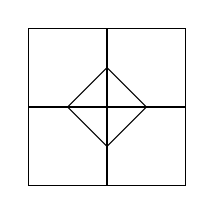
\begin{tikzpicture}
      \begin{scope}
        \draw (-1, -1) -- (1, -1) -- (1, 1) -- (-1, 1) -- (-1, -1);
        \draw (-0.5, 0) -- (0, -0.5) -- (0.5, 0) -- (0, 0.5) -- (-0.5, 0);
        \draw (0, -1) -- (0, 1);
        \draw (-1, 0) -- (1, 0);
      \end{scope}
    \end{tikzpicture}
  \end{figure}
\end{definition}

Each $k$-gon of the sequence $(k > 4)$ can be grouped together with $k-2$ triangles to create a ``flat'' block (they fullfill \autoref{eq:zero:curv:4}). This can be brought to a square form by adding $2 \times 2$ building blocks, as well as some additional triangles and pentagons as seen in the following picture.
\begin{definition}[Basic building block] The following will be called ``basic building block''.
  \begin{figure}[htpp]
    \centering
    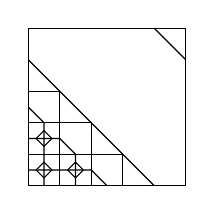
\begin{tikzpicture}[scale=0.1]
      \begin{scope}
        \draw (-10, -10) -- (10, -10) -- (10, 10) -- (-10, 10) -- (-10, -10);
        \draw (6, 10) -- (10, 6);
        \draw (6, -10) -- (-10, 6);
        \draw (2, -10) -- (2, -6) -- (-10, -6);
        \draw (-2, -10) -- (-2, -2) -- (-10, -2);
        \draw (-6, -10) -- (-6, 2) -- (-10, 2);
        \draw (2, -10) -- (2, -6) -- (-10, -6);
        \draw (-2, -10) -- (-2, -2) -- (-10, -2);
        \draw (-6, -10) -- (-6, 2) -- (-10, 2);
        \draw (-10, 0) -- (-8, -2) -- (-8, -10);
        \draw (-10, -4) -- (-6, -4) -- (-4, -6) -- (-4, -10);
        \draw (-10, -8) -- (-2, -8) -- (0, -10);
        \draw (-3, -8) -- (-4, -9) -- (-5, -8) -- (-4, -7) -- (-3, -8);
        \draw (-8, -3) -- (-9, -4) -- (-8, -5) -- (-7, -4) -- (-8, -3);
        \draw (-8, -7) -- (-9, -8) -- (-8, -9) -- (-7, -8) -- (-8, -7);
      \end{scope}
    \end{tikzpicture}
  \end{figure}
  Note that it has the form of a square, where the top and right as well as the bottom and left sides have the same amount of edges, which is even.
\end{definition}

\begin{definition}[Basic building block] The following will be called ``basic building block''.
  \begin{figure}[htpp]
    \centering
    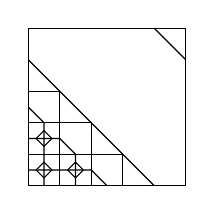
\begin{tikzpicture}[scale=0.1]
      \begin{scope}
        \draw (-10, -10) -- (10, -10) -- (10, 10) -- (-10, 10) -- (-10, -10);
        \draw (6, 10) -- (10, 6);
        \draw (6, -10) -- (-10, 6);
        \draw (2, -10) -- (2, -6) -- (-10, -6);
        \draw (-2, -10) -- (-2, -2) -- (-10, -2);
        \draw (-6, -10) -- (-6, 2) -- (-10, 2);
        \draw (2, -10) -- (2, -6) -- (-10, -6);
        \draw (-2, -10) -- (-2, -2) -- (-10, -2);
        \draw (-6, -10) -- (-6, 2) -- (-10, 2);
        \draw (-10, 0) -- (-8, -2) -- (-8, -10);
        \draw (-10, -4) -- (-6, -4) -- (-4, -6) -- (-4, -10);
        \draw (-10, -8) -- (-2, -8) -- (0, -10);
        \draw (-3, -8) -- (-4, -9) -- (-5, -8) -- (-4, -7) -- (-3, -8);
        \draw (-8, -3) -- (-9, -4) -- (-8, -5) -- (-7, -4) -- (-8, -3);
        \draw (-8, -7) -- (-9, -8) -- (-8, -9) -- (-7, -8) -- (-8, -7);
      \end{scope}
    \end{tikzpicture}
  \end{figure}
  Note that it has the form of a square, where the top and right as well as the bottom and left sides have the same amount of edges, which is even.
\end{definition}
